%%____________________________________________________________________________||
\section{Trigger strategy}
\label{sec:triggers}


\subsection{Hadronic signal region\label{sec:hadronic_signal_region}}

In Run~2 the RA1 analysis retains the low-thresholds of Run~1 with developments 
to the trigger selection, maintaining sensitivity to signatures of new physics with hadronic 
energies as low as $\scalht = 200$ GeV. This in part is achieved by a migration to PF-based 
jet reconstruction within the HLT which, in conjunction with a reduction of clustering radius 
parameter $\Delta R = 0.4$, provides improvements in jet energy resolution in high-pileup 
conditions and mitigates the effects of pileup contamination within the jet cone.

A suite of $\scalht$-$\alphat$ cross-triggers with a requirement on the minimum average \pt of 
the leading two jets, $\pt^{\rm \left<j1,j2\right>}$, are utilised in the selection of events in 
the hadronic signal region, labelled: \verb!HLT_PFHTXXX_PFDijetYYY_AlphaT0pZZ!. The use of a 
dijet average threshold provides an improved suppression of QCD multijet events within the trigger,
enabling looser \alphat thresholds to be utilised whilst maintaining acceptance to events exhibiting asymmetric jet 
topologies such as monojet-like signatures of compressed spectrum and DM models. 
It should be noted that for the asymmetric jet topologies, the use of a dijet average threshold of 90 \GeV
will result in certain events, where the leading jet \pt is soft in regards to a monojet-like signature, being
rejected. While it is possible to reduce the threshold of the dijet average and recover trigger efficiency,
it was not possible to ensure the rate of this lowered threshold remained low. It was found that a dijet average
threshold of 90 \GeV ensured the optimum performance when balancing efficiency and rate, with both the $\scalht$ and $\alphat$
thresholds. 

The Level-1 seeds for the HLT paths are given by the disjunction of the lowest 
unprescaled Level-1 hadronic scalar energy and missing energy sum seeds (\verb!HTTXXX_OR_ETMYYY!) for 
the given run scenario. A loose calorimeter trigger prefilter is utilised to reduce the pass-through 
rate prior to track-based 
reconstruction, ensuring the PF-based filters meet timing requirements. The calorimeter prefilter 
utilises loose \scalht and dijet average \pt requirements in addition to a new variable \alphat', 
defined as \alphat in the limit $\Delta\scalht \rightarrow 0$, which better correlates \alphat 
between calorimeter and PF-based reconstruction.

The thresholds of the signal triggers, shown in Table~\ref{tab:2015_Hadronic_Signal_Triggers}, are 
tuned to maintain acceptance for a range of signal topologies whilst effectively suppressing QCD 
multijet events to maintain acceptable trigger rates. These triggers uniquely seed individual offline \scalht 
bins with the exception of the highest-\scalht \scalht-\alphat cross-trigger which is utilised for analysis 
bins in the range: 
$400 < \scalht < 800$ \GeV. Above $\scalht > 800$ a pure \scalht trigger, \verb!HLT_PFHT800!, is utilised 
which has no explicit dependence on $\alphat$ or dijet average threshold. These triggers form the primary 
signal selection menu, in addition a set of secondary triggers with higher \alphat thresholds provide redundancy 
for higher luminosity scenarios. 

% TABLE : 2015 triggers
%----------------------------------------------------------------------
\begin{table}[h!]
\topcaption{Trigger thresholds of the Level-1, calorimeter prefilter and final PF-trigger decision for
 the primary HLT paths for the hadronic signal region in the $\lumi=7\times10^{33}\cm^{-2}{\rm s}^{-1}$ scenario.
 Higher threshold Level-1 \scalht and \met seeds are utilised for the higher luminosity scenario. }
\footnotesize
\centering
\begin{tabular}{c|cccc} 
\hline
\hline
HLT path     & L1 seed & HLT calo-prefilter & HLT PF-filter                                                \\
    &        & ($\scalht$, $\alphat$', $\pt^{\rm \left<j1,j2\right>}$) & ($\scalht$, $\alphat$, $\pt^{\rm \left<j1,j2\right>}$) \\ %& (Hz) \\[0.7 ex] 
\hline
 \verb!HLT_PFHT200_PFDijetAve90_AlphaT0p57! & \verb!HTT125 OR ETM50! & 150, 0.540, 70 & 200, 0.570, 90 \\ %& \\ % 11.0 $\pm$ 3.0 \\
 \verb!HLT_PFHT250_PFDijetAve90_AlphaT0p55! & \verb!HTT125 OR ETM50! & 200, 0.535, 70 & 250, 0.550, 90 \\ %& \\ % 8.5  $\pm$ 3.0 \\
 \verb!HLT_PFHT300_PFDijetAve90_AlphaT0p53! & \verb!HTT125 OR ETM50! & 250, 0.525, 70 & 300, 0.530, 90 \\ %& \\ % 9.5  $\pm$ 3.0 \\
 \verb!HLT_PFHT350_PFDijetAve90_AlphaT0p52! & \verb!HTT125 OR ETM50! & 300, 0.520, 70 & 350, 0.520, 90 \\ %& \\ % 10.0 $\pm$ 3.0 \\
 \verb!HLT_PFHT400_PFDijetAve90_AlphaT0p51! & \verb!HTT125 OR ETM50! & 370, 0.510, 70 & 400, 0.510, 90 \\ %& \\ % 13.5 $\pm$ 3.5 \\ \\ %\hline \\ %
 \verb!HLT_PFHT800!                         & \verb!HTT175!          & 650, -, -      & 800, -, -      \\ %& \\ % 13.5 $\pm$ 3.5 \\ \\ %\hline \\ %
\hline
\hline
\end{tabular}
\label{tab:2015_Hadronic_Signal_Triggers}
\end{table}

The efficiency of the signal triggers is determined using both
simulation and data samples. Data-driven measurements are performed with an electron sample, selected by the
unprescaled \verb!HLT_Ele23_eta2p1_WPLoose_Gsf! reference trigger. To remain consistent with the reconstruction 
of electrons in the trigger, no cross-cleaning of electrons from jets are performed offline, with
the electron being included in the computation of event variables.

Based on simulation studies, the signal triggers demonstrate high
efficiencies for a range of benchmark signal models and SM processes
with genuine \met. The trigger efficiency for two benchmark signal
models, \texttt{T2tt} (425,325) and \texttt{T1tttt} (1200,800), are
shown in Figure~\ref{fig:T1ttt_Trigger_Efficiency} for the low and
high jet multiplicity analysis bins, respectively, which illustrate a
``representative'' performance for each of the respective models.
  
The use of a dijet average threshold is fully efficient for the
categories with ``symmetric'' \Pt selection requirements on the
leading two jets, as illustrated in
Fig.~\ref{fig:T1ttt_Trigger_Efficiency_DijetAve}. In the case of the
``asymmetric'' scenario, when the second leading jet satisfied $40 <
\Pt < 100\gev$, some inefficiencies are observed due to this
challenging class of event, where both the leading and second jet
are relatively soft and the \scalht is low. The figure shows the
efficiencies for the lowest \scalht bin, $200 < \scalht < 250\gev$, 
which improve significantly for the higher \scalht bins in the region
$\scalht < 250\gev$. 

However, an important goal of the analysis is to have good acceptance
to compressed SUSY and general DM models. It is therefore critical
that we operate in the trigger turn on regions for the lower
thresholds. We have already successfully exercised this approach with
the Run~1 analysis and are thus confident that we can do this again
during Run~2. As in Run~1, multiple efficiency measurements are
employed, which are performed with data and propagated through to the
analysis with cross checks in simulation.

However, it is noted that for the majority of models accessible by the
"Early Analysis", such as gluino-induced production and decay, the
most sensitive bins are typically at higher values of MHT, for which
the triggers perform close to full efficiency. Lower MHT bins will be
subject to trigger efficiency corrections based on measurements in
data, as discussed above. 


% FIGURE: Trigger efficiencies
%----------------------------------------------------------------------
\begin{figure}[h!]
  \begin{center}
    \subfigure[$\njet = 2$]   {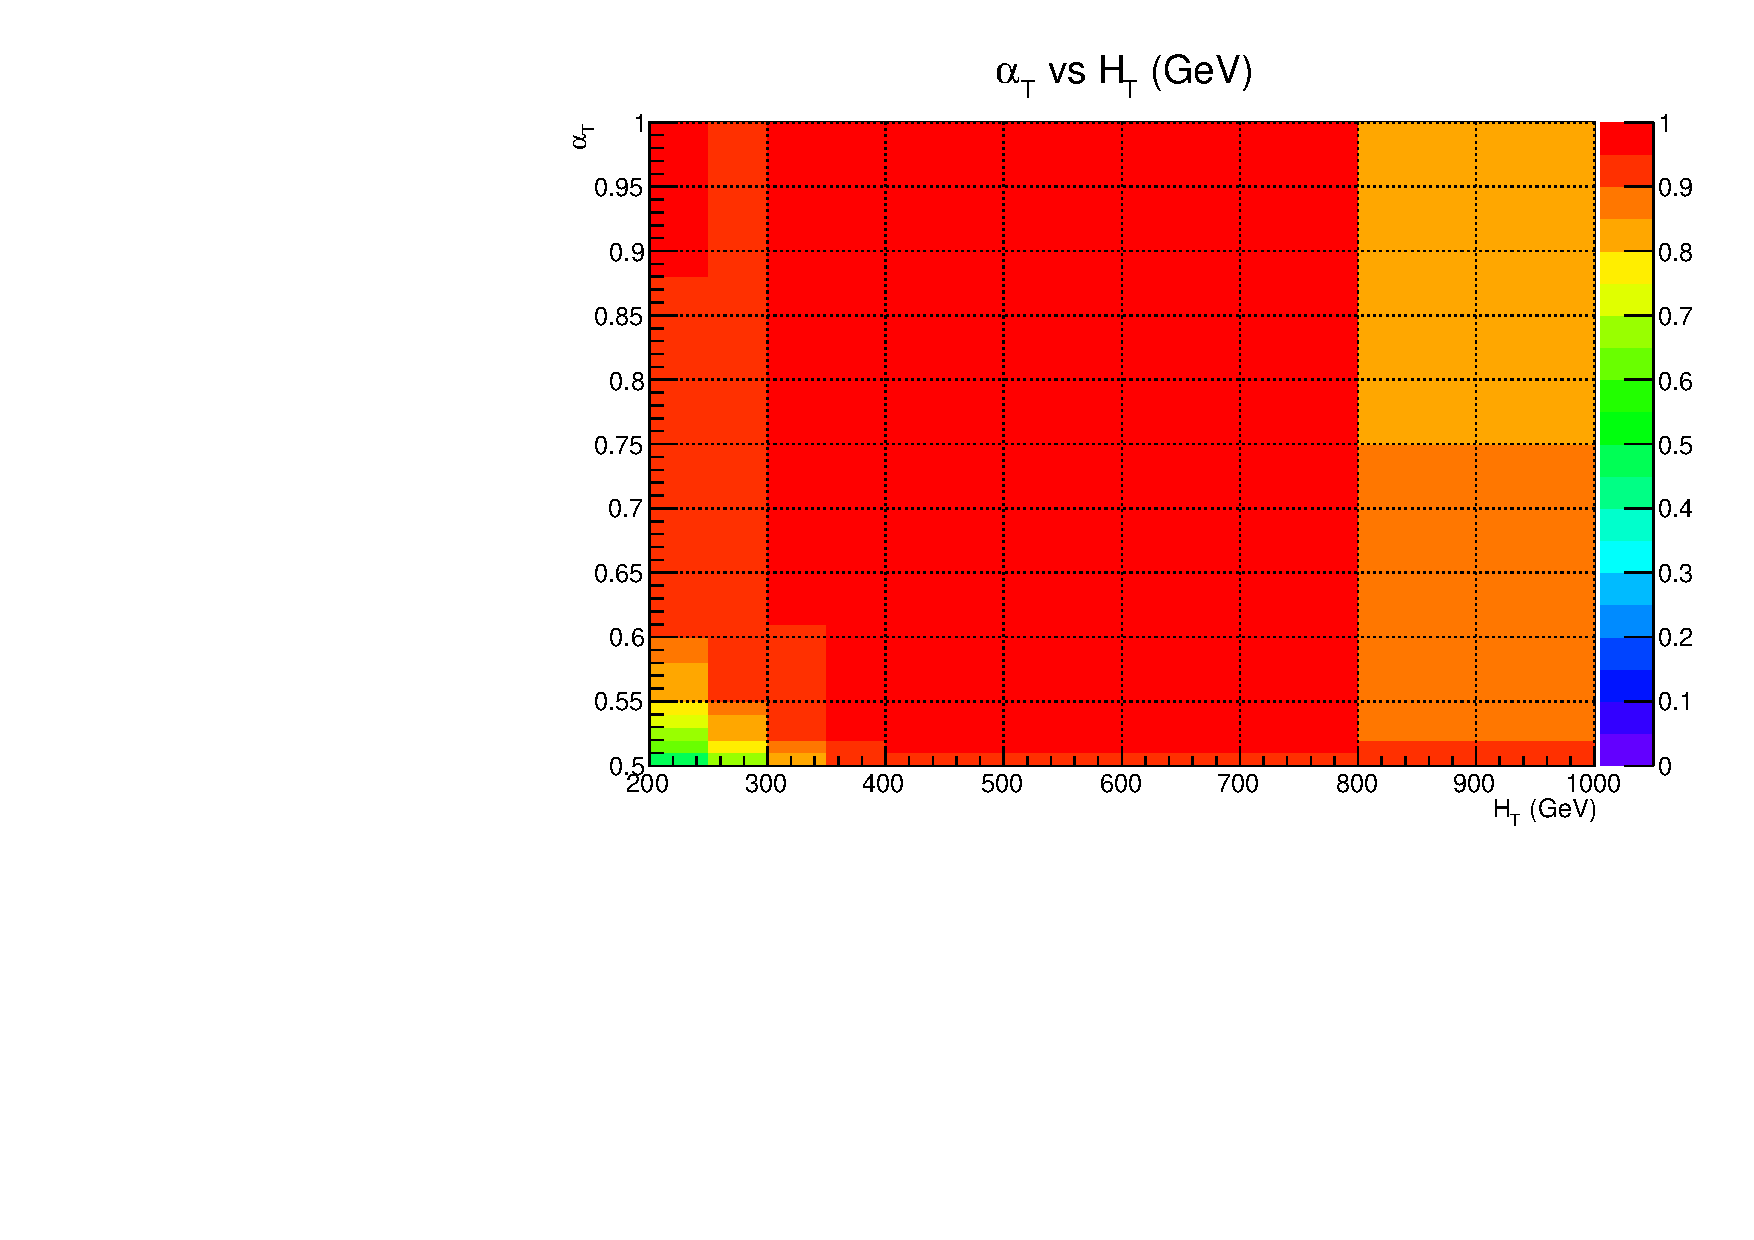
\includegraphics[width=0.5\textwidth]{figures/Trigger/T2tt_425_325_eq2j_ht_vs_alphaT_Cumul.pdf}} ~~
    \subfigure[$\njet \geq 5$]{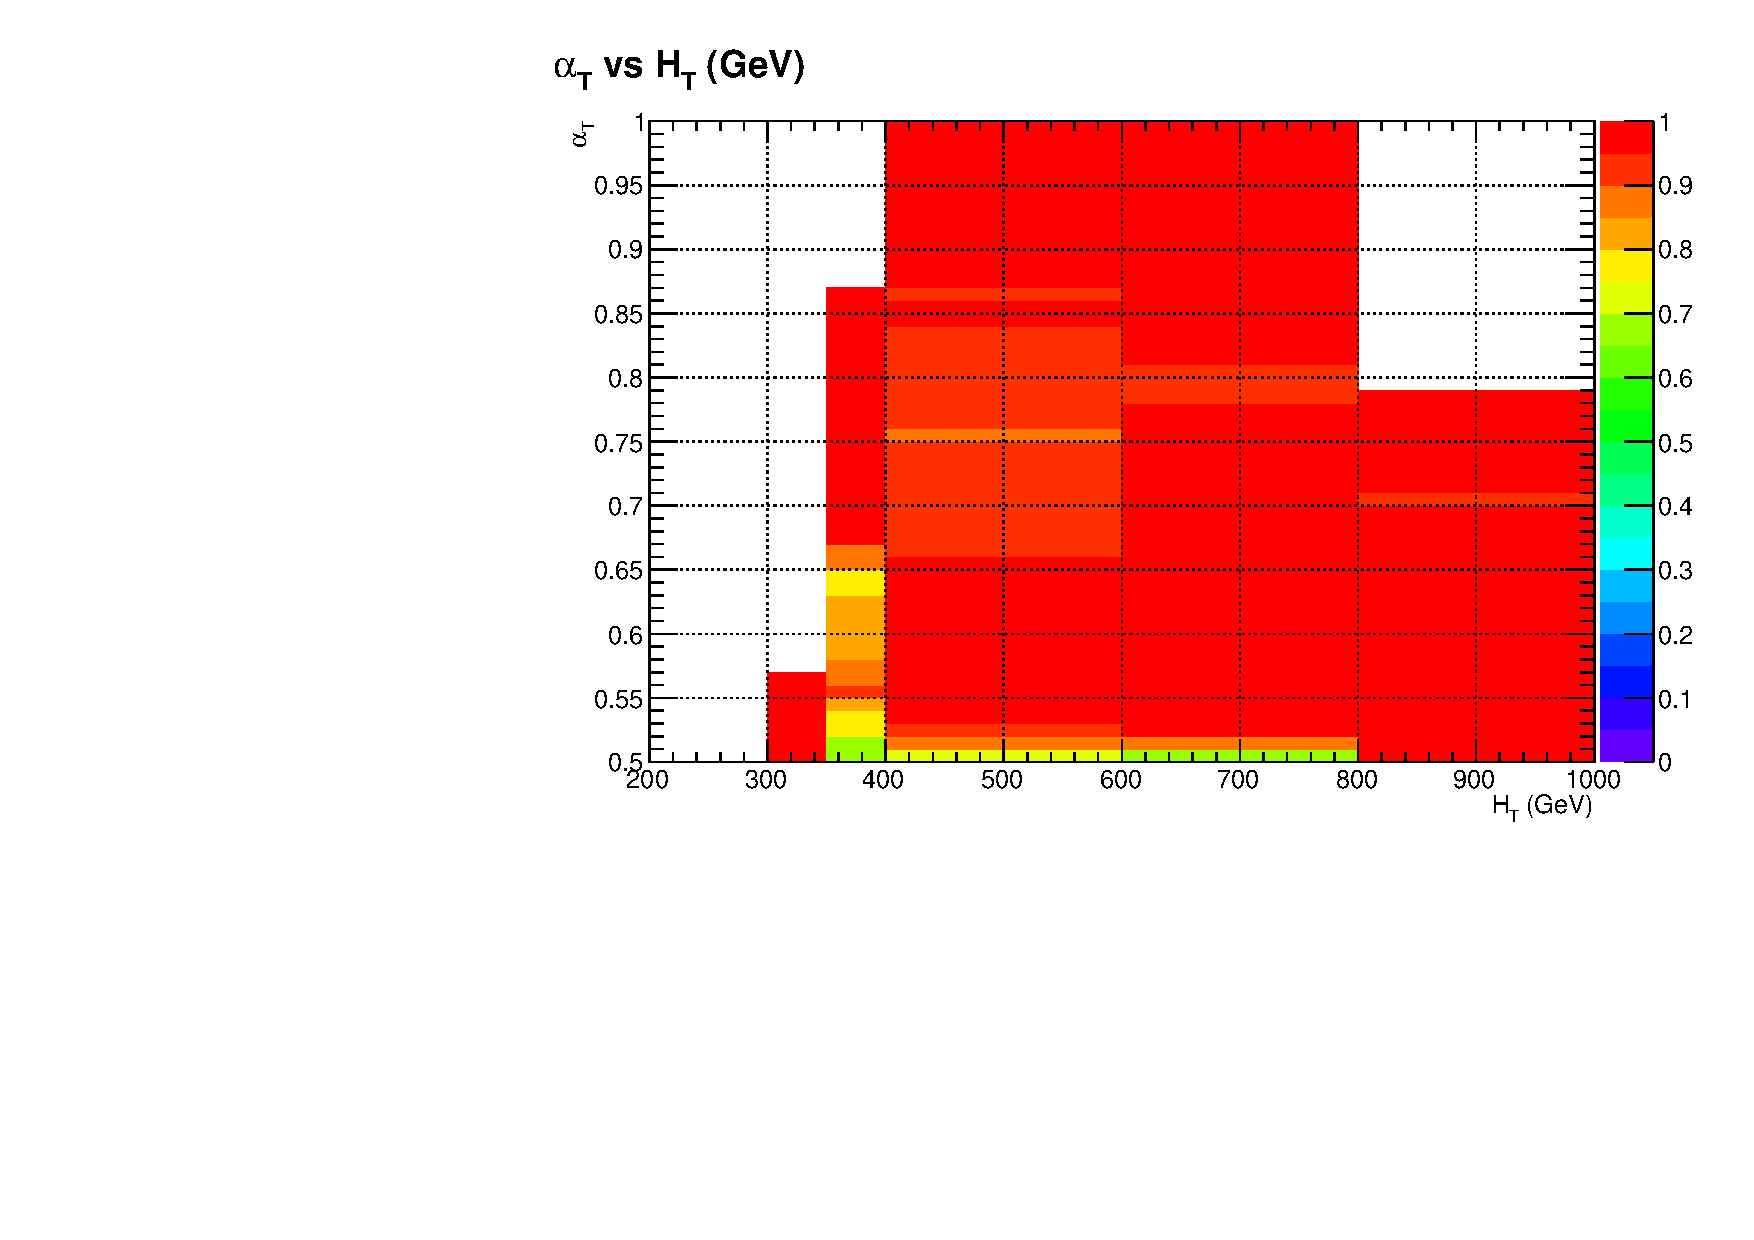
\includegraphics[width=0.5\textwidth]{figures/Trigger/T1tttt_1200_800_ge5j_ht_vs_alphaT_Cumul.pdf}} \\
    \subfigure[$\njet \geq 2$]   {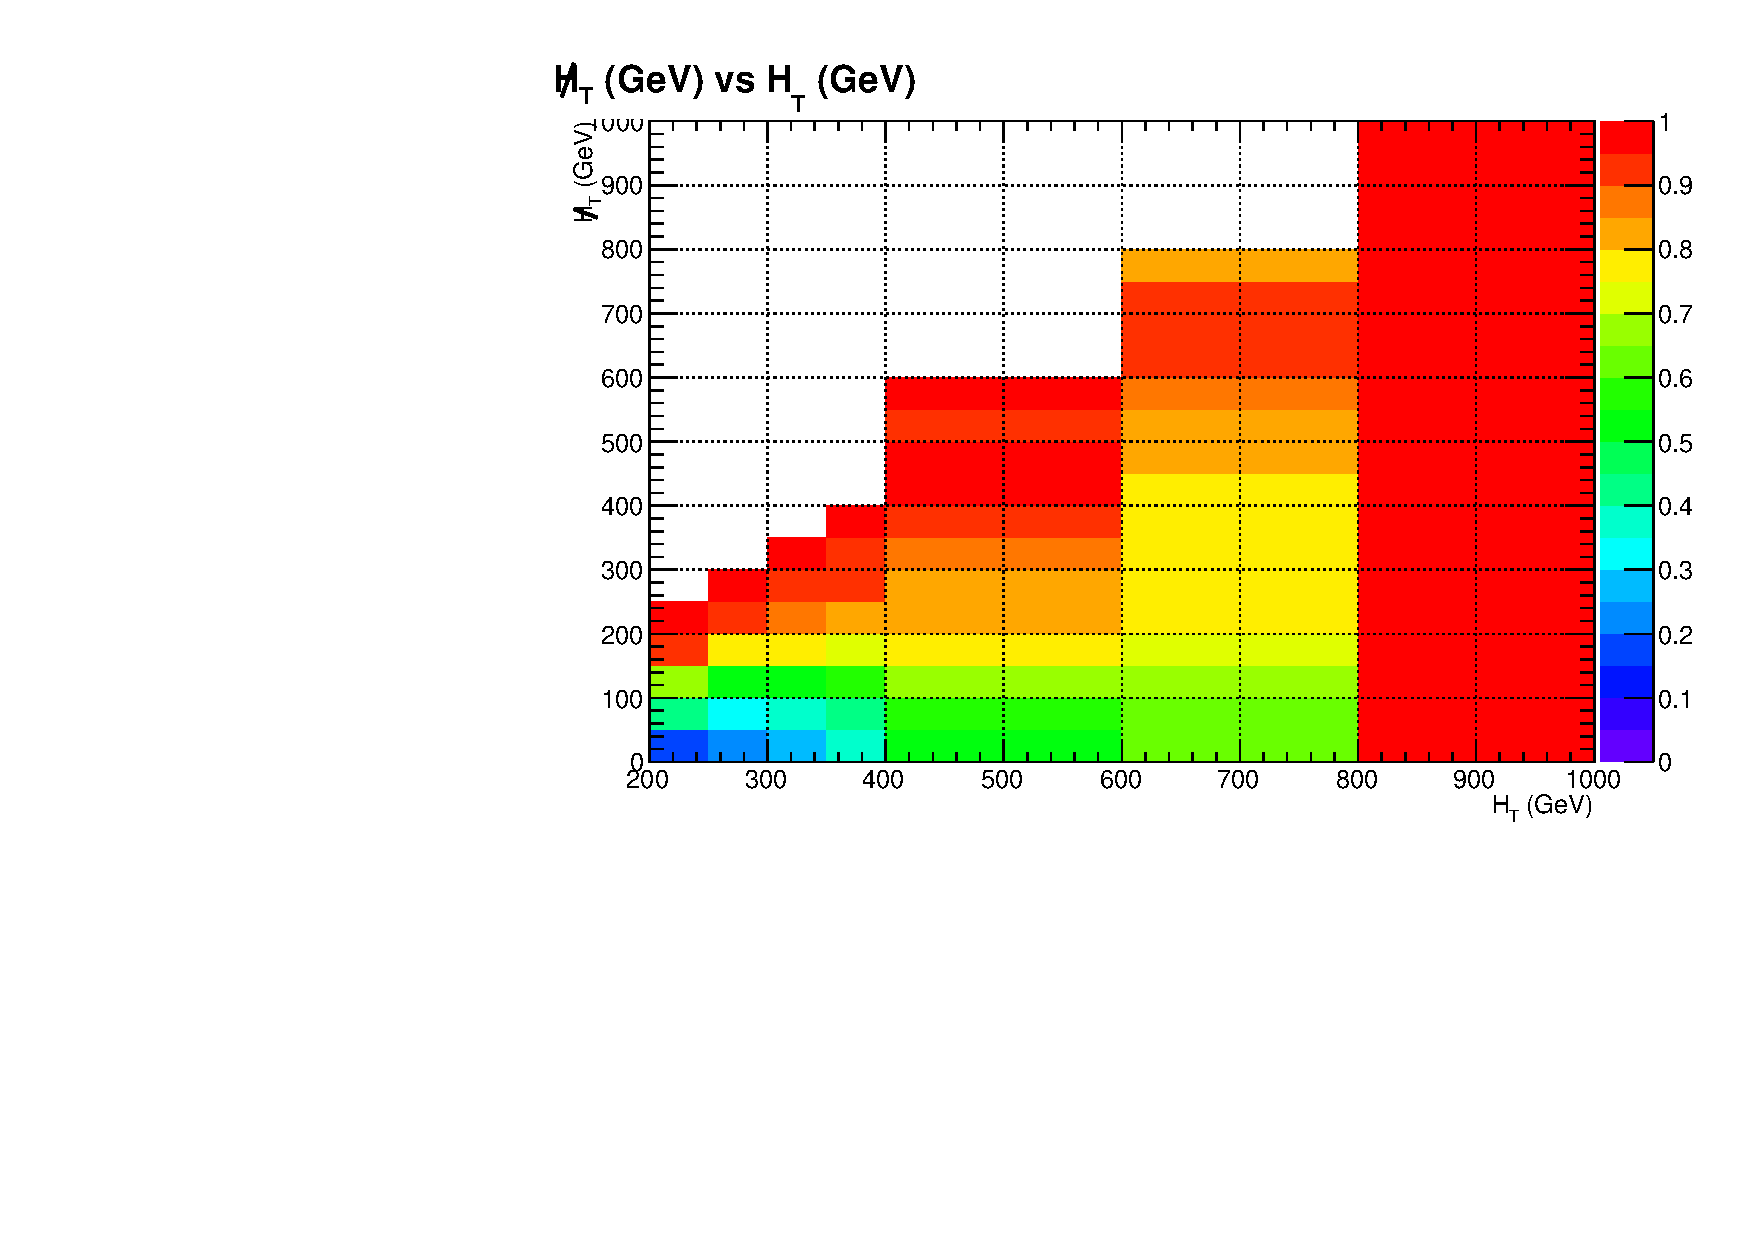
\includegraphics[width=0.5\textwidth]{figures/Trigger/T2tt_425_325_Sym_ht_vs_mht_Cumul.pdf}} ~~
    \subfigure[$\njet \geq 5$]{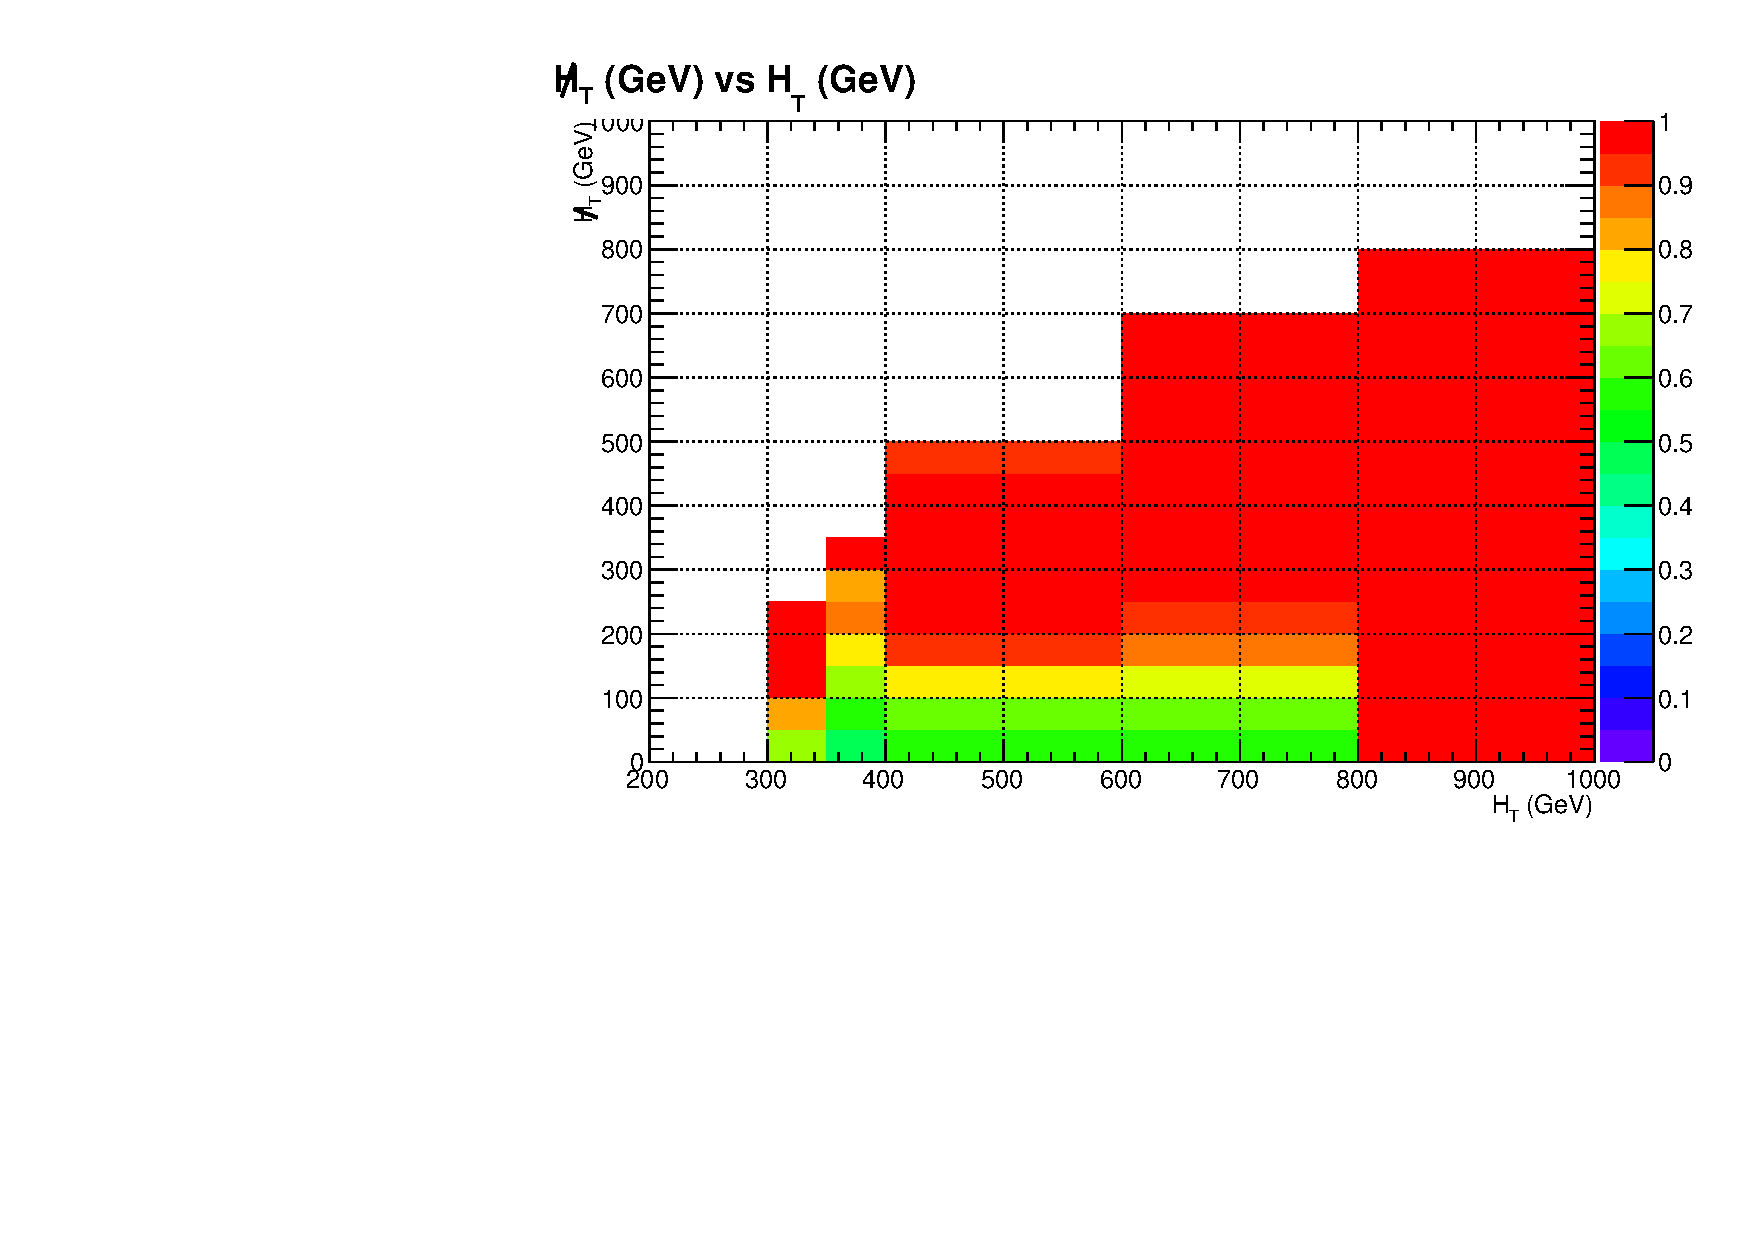
\includegraphics[width=0.5\textwidth]{figures/Trigger/T1tttt_1200_800_ge5j_ht_vs_mht_Cumul.pdf}} \\
    \caption{
Cumulative trigger efficiency for the T2tt(425,325) and T1tttt(1200,800) simplified models after signal selection in the \alphat-\scalht and \mht-\scalht planes for representative analysis jet multiplicity bins.}
    \label{fig:T1ttt_Trigger_Efficiency}
  \end{center} 
\end{figure}


% FIGURE: Trigger efficiencies - Dijet average
%----------------------------------------------------------------------
\begin{figure}[h!]
  \begin{center}
    \subfigure[Symmetric-$\njet$ requirement]  {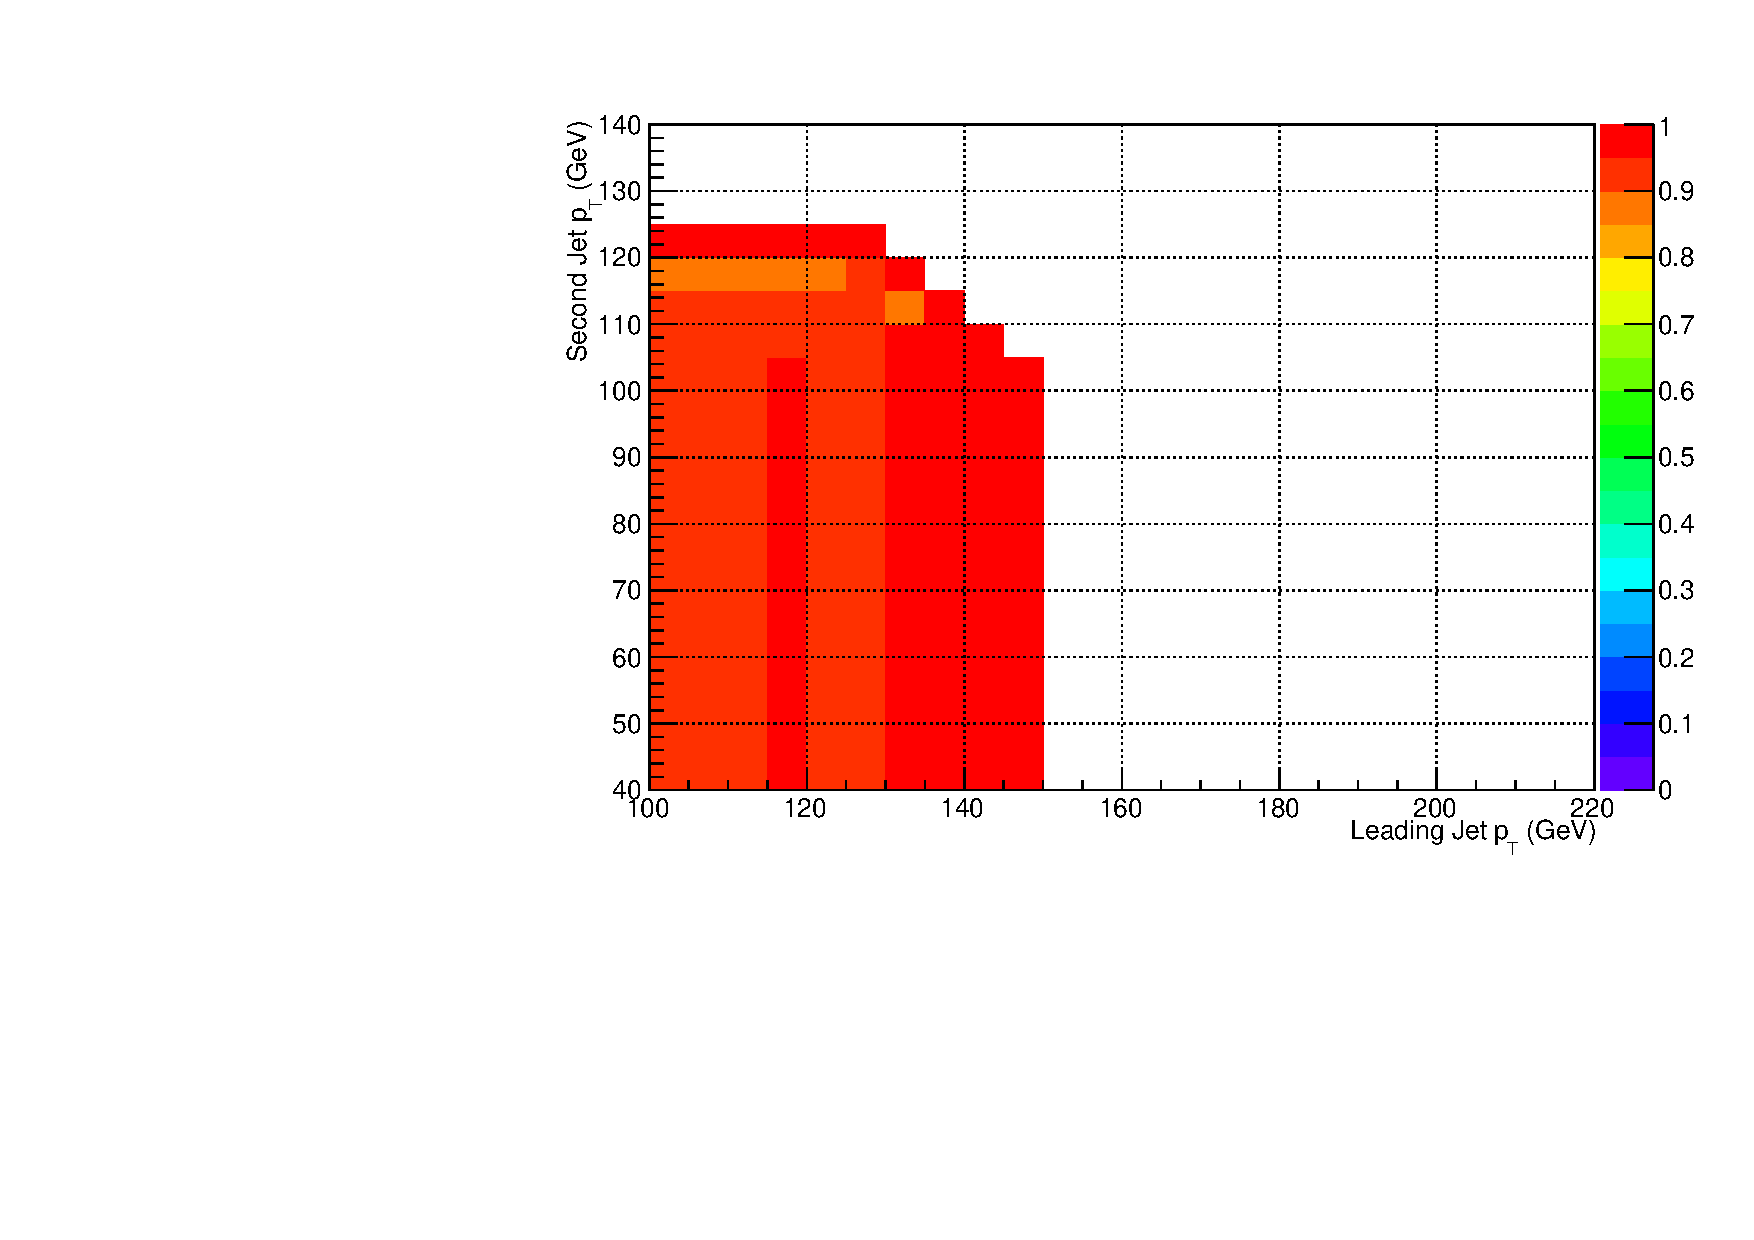
\includegraphics[width=0.5\textwidth]{figures/Trigger/T2tt_425_325_Sym_j1vsj2_cumulEff.pdf}} ~~
    \subfigure[Asymmetric-$\njet$ requirement]{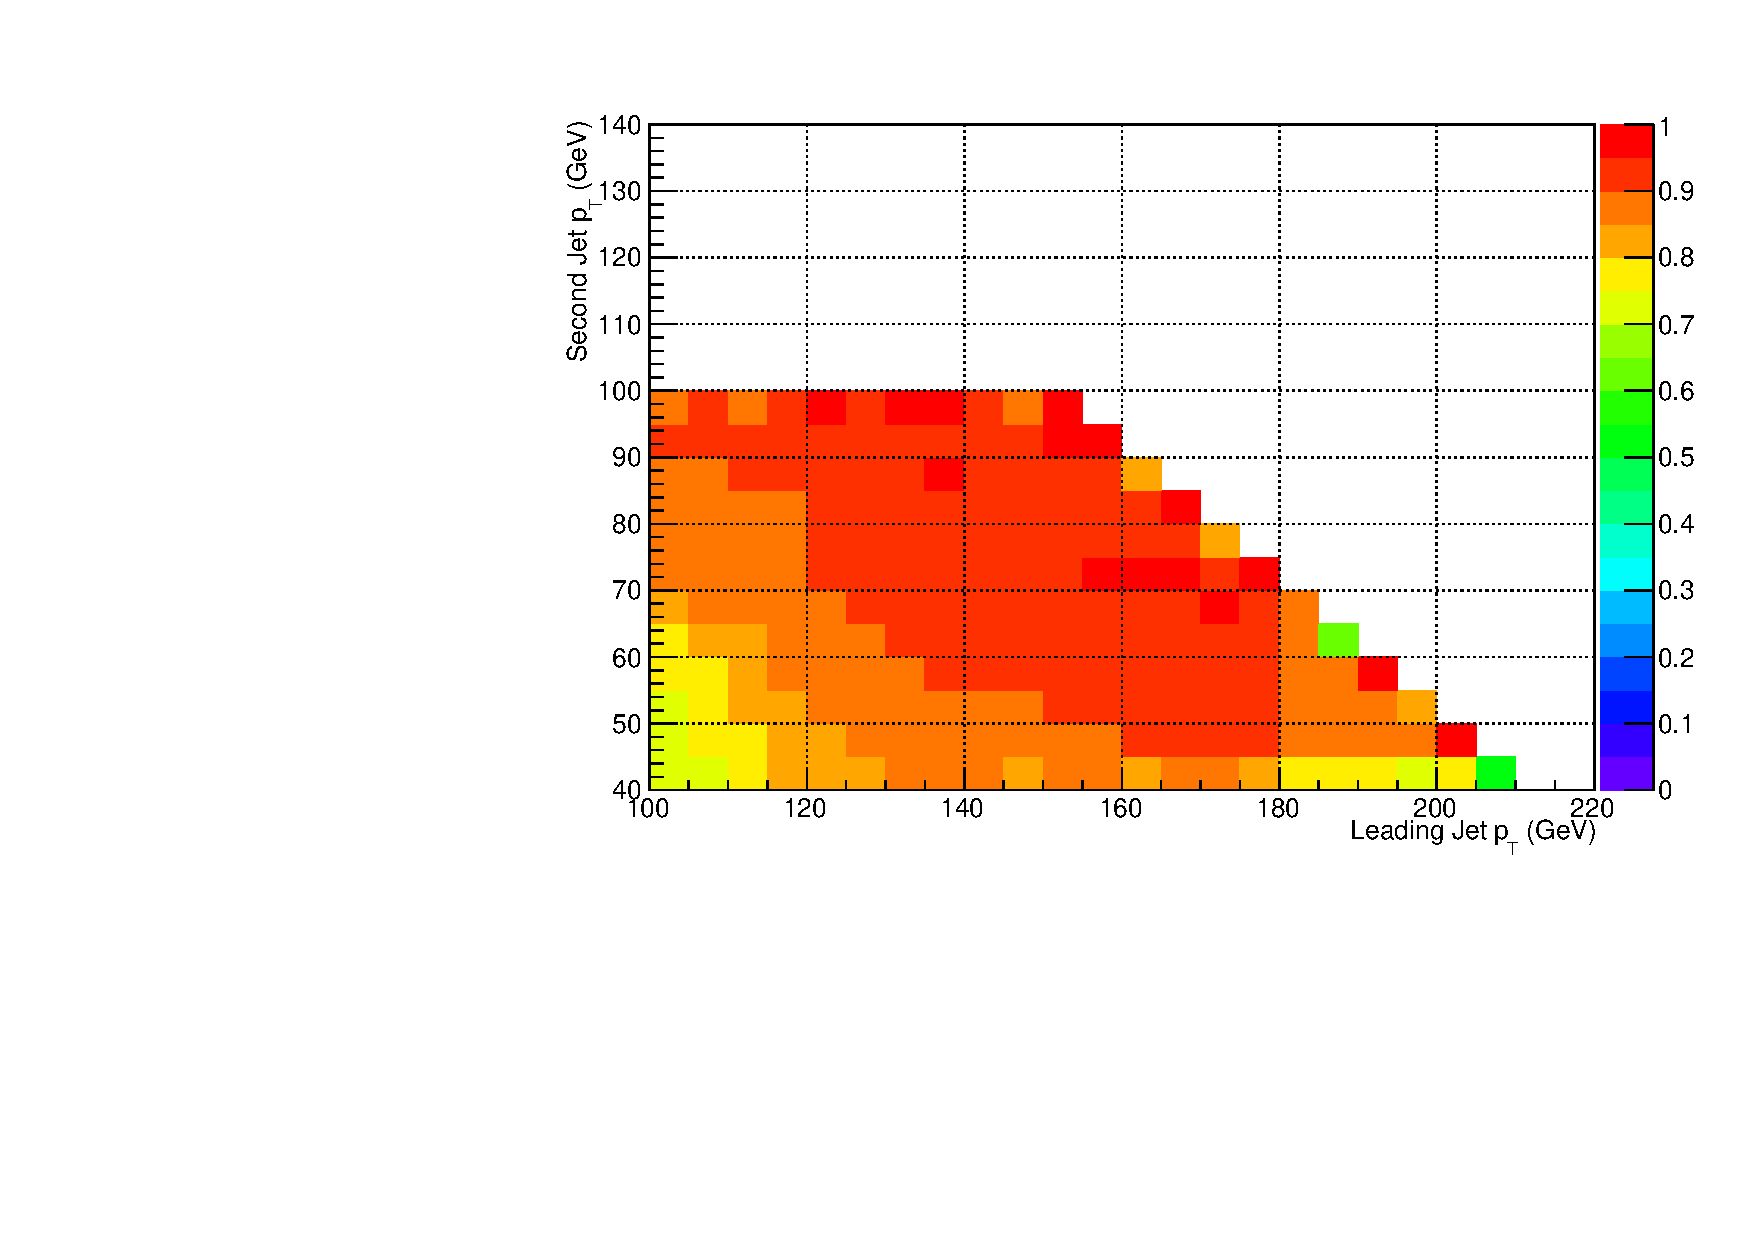
\includegraphics[width=0.5\textwidth]{figures/Trigger/T2tt_425_325_Asym_j1vsj2_cumulEff.pdf}} \\
    \caption{
Cumulative trigger efficiency for the T2tt(425,325) simplified model after signal selection as a function of leading and second jet threshold for the symmetric and asymmetric selection requirements for the lowest-\scalht bin.}
    \label{fig:T1ttt_Trigger_Efficiency_DijetAve}
  \end{center} 
\end{figure}





% Control region triggers
\subsection{Control samples\label{sec:control_samples}}
Prescaled $\scalht$ triggers, \verb!HLT_HTXXX!, and a prescaled 
$\scalht$-$\alphat$ cross-trigger, are utilised in the 
selection of events for the hadronic control region. Shown 
in Table~\ref{tab:2015_Hadronic_Control_Triggers} these triggers share the same Level-1 
seeds and $\scalht$ threshold of the signal cross-triggers and are similarly each mapped 
to a unique offline bin. The efficiency of these triggers are similarly measured from an electron 
reference trigger in addition to an independent measurement with the \verb!HLT_Physics! 
minimum bias trigger.


% TABLE: Hadronic control region
%----------------------------------------------------------------------
\begin{table}[h!]
\topcaption{Hadronic control triggers. }
\footnotesize
\centering
\begin{tabular}{c|cc} 
\hline
\hline
HLT path & \multicolumn{1}{c}{Prescale} \\
\hline
\texttt{HLT\_PFHT200} & 3060 \\
\texttt{HLT\_PFHT250} & 2040 \\
\texttt{HLT\_PFHT300} & 1020 \\
\texttt{HLT\_PFHT350} & 180  \\
\texttt{HLT\_PFHT400} & 120  \\
\texttt{HLT\_PFHT200\_PFAlphaT0p51} & 175 \\
\hline
\hline

\end{tabular}
\label{tab:2015_Hadronic_Control_Triggers}
\end{table}


The non-hadronic control regions are seeded by the lowest-threshold unprescaled 
triggers available in the given run scenario. In the high-luminosity scenario The 
\mj and \mmj control samples are selected with the \verb!HLT_IsoMu20! trigger,
and the \gj control sample by the \verb!HLT_Photon125! trigger. The \ej and \eej
control samples may be seeded by the \verb!HLT_Ele23_eta2p1_WPLoose_Gsf! trigger.

The efficiency of the control triggers will be measured with data-driven methods
(provided by the relevant POG). The tag and probe method is used in the measurement of
efficiencies of the muon and electron triggers and a loose photon reference trigger 
is utilised in the measurement of the photon trigger efficiency. For the results in 
this note for the muon control regions the emulated trigger bit in MC is used to simulate 
the trigger. An offline \Pt requirement of 200\GeV is made on the photon
to ensure it is in the efficiency plateau of the trigger.








\subsection{Low-$\scalht$ Level-1 seeds}

Some models of new physics, such as supersymmetric compressed spectrum models, are challenging to select at the trigger level due to low-hadronic energy visible in the final state. Sensitivity to such models require low trigger thresholds which is difficult to achieve without incurring a large increase in the Level-1 trigger rate. New Level-1 seeds which enable low thresholds to be utilised by actively vetoing QCD event topologies have been studied and are shown to have higher efficiencies for such models than can be achieved with the current Level-1 menu.

The $\Delta\phi(j_{1}^{L1},j_{2}^{L1})$ seed exploits the typical dijet topologies exhibited in QCD dijet production by vetoing events where the azimuthal separation of the leading jets exceeds eight calorimeter regions, corresponding to a veto of: $\Delta\phi(j_{1}^{L1},j_{2}^{L1}) \ge 160^{\circ}$, where a jet threshold of $\pt > 32$ GeV is imposed on the second jet. This enables a much lower threshold on the $\scalht$-leg to be achieved, with a small increase in other thresholds in the menu, enabling for example the rate neutral trigger: \verb!L1_DoubleJetC32_WdPhi7_HTT125! to be utilised.

An alternate $\mht/\scalht$ 'reduced-MHT' seed exploits the correlation in missing hadronic energy and visible hadronic energy typical of decays with genuine $\met$ and the decorrelation of these quantities for QCD with fake-$\met$ by requiring a minimum $\mht/\scalht$ ratio. This again enables triggers with a significant reduction in the threshold on the $\scalht$-leg, for example with the rate neutral trigger: \verb!L1_HTT125_rHTM0p3!.

The logical disjunction of these two seeds can further improve signal efficiency whilst maintaining an effective suppression of QCD events by increasing acceptance to additional topologies. ISR-dominated final states for instance typically have large $\mht/\scalht$ but may fail the $\Delta\phi(j_{1}^{L1},j_{2}^{L1})$ selection, where as events with high jet multiplicities typically have high $\Delta\phi(j_{1}^{L1},j_{2}^{L1})$ but may fail the $\mht/\scalht$ threshold due to the breakdown in $\mht/\scalht$ at high jet multiplicities. Combined these seeds allow even smaller thresholds to be used on the $\scalht$-leg without loss of efficiency to ISR-dominated or high jet multiplicity events, for example with the trigger:\\ \verb!L1_HTT110_rHTM0p6_rHTM0p0_WdPhi6!.

The new trigger seeds can be implemented in the trigger hardware by repurposing the bits currently utilised for $\mht$ and $\phi({\mht})$ trigger primitives with the new $\mht/\scalht$ and $\Delta\phi(j_{1}^{L1},j_{2}^{L1})$ primitives respectively. These changes have been discussed with trigger experts and are deemed to be relatively simple to implement in the calorimeter trigger firmware and will have little impact on the operation global trigger. The latest version of the Level-1 trigger emulator currently has the \verb!L1_DoubleJetC32_WdPhi7_HTT125!, \verb!L1_HTT125_rHTM0p3! and \\ \verb!L1_HTT110_rHTM0p6_rHTM0p0_WdPhi6! low-$\scalht$ trigger primitives implemented, enabling a wider study within the collaboration.

The performance after the full offline selection of the low-$\scalht$ Level-1 seeds was studied for a range of signal models in the lowest $\scalht$ and $\njet$ analysis bins which are predominantly populated by compressed models. Performance was measured relative to the current PU40bx25 Level-1 hadronic menu, {\verb!HTT175! \verb!OR! \verb!DoubleJetC100! \verb!OR! \verb!QuadJetC60! \verb!OR! \verb!ETM70!}, with the rate equivalent low-$\scalht$ menues defined as: Low-$\scalht$ seed {\verb!OR! \verb!HTT200! \verb!OR! \verb!DoubleJetC120! \verb!OR! \verb!QuadJetC60! \verb!OR! \verb!ETM70!}. The efficiencies of the proposed menues for $\njet = 2$ and $\njet = 3$, shown in Table~\ref{tab:LowHT_Seed_Signal_2Jet} and Table~\ref{tab:LowHT_Seed_Signal_3Jet} respectively, show significant improvements in trigger efficiency utilising the low-$\scalht$ seeds with respect to the current hadronic menu and similar performance to what could be obtained by reducing the $\met$ threshold without the additional 3 kHz Level-1 trigger rate this would incur.

It is important to note that the new L1 seeds discussed in this
section are currently only potential alternatives to the existing L1
\texttt{ETM} and \texttt{HTT} seeds. Their inclusive may require some
rate balancing within the existing menus at the expense of other
seeds. Studies have considered the re-allocation of rate ($\sim$5~kHz)
from the \texttt{DoubleJetC} seed. The inclusion of these new seeds
may be a beneficial strategy to employ if the thresholds on the
\texttt{ETM} and \texttt{HTT} seeds are to be raised due to increasing
instantaneous luminosity and/or pileup conditions later in the run of
2015.

% TABLE : Low-HT seed efficiencies - NJet = 2
%----------------------------------------------------------------------
\begin{table}[h!]
\topcaption{Trigger efficiency for $\njet = 2$, $200 < \scalht \le 300$ analysis bin and corresponding rate of the current Level-1 hadronic menu and proposed low-$\scalht$ trigger menues for a range of compressed signal models.} %sparticle and LSP masses represented by the first and second bracketed term respectively.}
\footnotesize
\centering
\begin{tabular}{cccccc} 
\hline
\hline
  Signal model & Hadronic menu & $\Delta\phi(j_{1}^{L1},j_{2}^{L1})$ & $\mht/\scalht$ &$\Delta\phi(j_{1}^{L1},j_{2}^{L1})$ \verb!OR! $\mht/\scalht$ & Hadronic menu \verb!OR ETM60! \\
\hline
  T2cc(250, 210)   & 0.60 & 0.86 & 0.91 & 0.94 & 0.95 \\
  T2qq(400, 400)   & 0.63 & 0.82 & 0.88 & 0.95 & 0.94 \\
  T2tt(300, 200)   & 0.53 & 0.91 & 0.95 & 0.99 & 0.96 \\
\hline
  Menu rate (kHz) & 15   & 15   & 15   & 15   & 19   \\
\hline
\hline
\end{tabular}
\label{tab:LowHT_Seed_Signal_2Jet}
\end{table}

% TABLE : Low-HT seed efficiencies - NJet = 3
%----------------------------------------------------------------------
\begin{table}[h!]
\topcaption{Trigger efficiency for $\njet = 3$, $200 < \scalht \le 300$ analysis bin and corresponding rate of the current Level-1 hadronic menu and proposed low-$\scalht$ trigger menues for a range of compressed signal models.} %sparticle and LSP masses represented by the first and second bracketed term respectively.}
\footnotesize
\centering
\begin{tabular}{cccccc} 
\hline
\hline
  Signal model & Hadronic menu & $\Delta\phi(j_{1}^{L1},j_{2}^{L1})$ & $\mht/\scalht$ &$\Delta\phi(j_{1}^{L1},j_{2}^{L1})$ \verb!OR! $\mht/\scalht$ & Hadronic menu \verb!OR ETM60! \\
\hline
  T2cc(250, 210)   & 0.45 & 0.74 & 0.74 & 0.83 & 0.94 \\
  T2qq(400, 400)   & 0.46 & 0.88 & 0.88 & 0.93 & 0.92 \\
  T2tt(300, 200)   & 0.41 & 0.76 & 0.83 & 0.84 & 0.86 \\
\hline
  Menu rate (kHz) & 15   & 15   & 15   & 15   & 19   \\
\hline
\hline
\end{tabular}
\label{tab:LowHT_Seed_Signal_3Jet}
\end{table}



%%____________________________________________________________________________||
